% GENERATED FROM typst/manual/sections/03_short_window_rcd_shedding_fixtures.typ BY scripts/typ2tex.py (v1.0.0) — DO NOT EDIT.
% Edit canonical Typst under typst/ and regenerate with: python3 scripts/typ2tex.py --root . --outdir latex

\section{Exact Internal Fixtures}\label{manual:cross-return-short-window}

\paragraph{Setup and calculation card.}
Declared gates, windows, and signed integer bins determine the slit accounting
identity and exact $\delta_3$ residuals (\texttt{RC-030}); declared motif support,
channel capacity, and closure targets determine clipped pressure, pending overhang,
and shedding surplus (\texttt{RC-038}). All evaluations are conditional exact
zero-float arithmetic under \secref{manual:calculation-spine}. These tables supply
internal comparators and falsifiers---never an empirical probability law or a routed
lifetime prediction.

\aodnoteblock{Scope}{This section carries exact A$\Omega$-internal fixtures: Dimonhexon double-slit cross-return, short-window duration-clipping, exact $\delta_3$ residual tallies, and sheddic route audits.}

\aodnoteblock{Data-support class}{These are D0 exact internal fixtures. Inputs are declared integer gates, channels, windows, and comparator bins. Comparator fixtures record $O_k,\Delta^{\mathbb{Z}}_k,\delta_{3,k}$; route-audit fixtures record $\Delta_{\mathrm{close}}$, $X_{\mathrm{shedding}}$, and $\operatorname{SheddicPath}$.}

\subsection{Dimonhexon cross-return fixture}\label{manual:cross-return:dimonhexon-slit}

\aodnoteblock{Scope}{This subsection is a boundary-restriction test: a stable Dimonhexon closure enters a slit boundary, undergoes duon-cycle handoff across the restricted boundary/window, and recloses into target bins.}

\aodprovenance{\mainsection{main:subsec:fractal-field-ring-gate};
\mainequation{main:eq:sadar-operator-cycle}.}

\paragraph{Setup.}
Declare the slit scope and carried form:

\[
\mathbf{a}_{\mathrm{slit}}\vdash(F_{1:2:6},R_{\mathrm{slit}},\partial R_{\mathrm{slit}},\omega_{\mathrm{slit}}),\qquad B_{\mathrm{slit}}=(\partial F_{1:2:6},\omega_{\mathrm{slit}}),
\]

\[
1:2:6=\mathrm{Dimonhexon}.
\]

The boundary-restricted handoff follows the exact chain

\[
\mathrm{Dimonhexon}\longrightarrow W_{\omega}[D_i\mu D_j]\longrightarrow\Delta^{\chi\mathrm{lag}}\longrightarrow\mathbf{A}_F(B_{\mathrm{slit}})\longrightarrow\text{local reclosure bins}.
\]

For one gate $g_a$ and target bin $k\in K_{\mathrm{bin}}$, summing over the bound
discrete-window cut index $t\in\omega$ (kept strictly distinct from the bin index $k$)
gives the one-gate contribution

\[
S^{(a)}_k=\sum_{t\in\omega}\sum_{\gamma:g_a\leadsto k}\kappa_k\SADARop_{B|t}(C_{\gamma}),
\]

with $S^{(b)}_k$ defined analogously for the second gate $g_b$.

\aodremark{Retained closure supplies the particle-like term, boundary-constrained handoff supplies the wave-like term, and local reclosure supplies the hit-like term.}

\subsection{Recurrent-ring double-slit cross-return}\label{manual:cross-return:ring-double-slit}

\aodnoteblock{Scope}{This subsection applies the main-note fractal field ring gate to the Dimonhexon slit handoff.}

\paragraph{Setup.}
Declare the recurrent ring field on cyclic vertex set $V_N$ and adjacency $E_N$:

\[
\mathbf{a}_{\mathrm{ring}}\vdash(F_{\mathrm{ring}},R_{\mathrm{ring}},\partial R_{\mathrm{ring}},\omega_{\mathrm{ring}}),\qquad B_{\mathrm{ring}}=(\partial_TF_{\mathrm{ring}},\omega_{\mathrm{ring}}),
\]

\[
V_N=\{0,1,\dots,N-1\},\qquad E_N=\{(i,i+1\bmod N),(i,i-1\bmod N):i\in V_N\}.
\]

Fix two boundary gates and the discrete target-bin set:

\[
g_a,g_b\in\partial_TR_{\mathrm{ring}},\qquad k\in K_{\mathrm{bin}}.
\]

\begin{figure}[H]
\centering
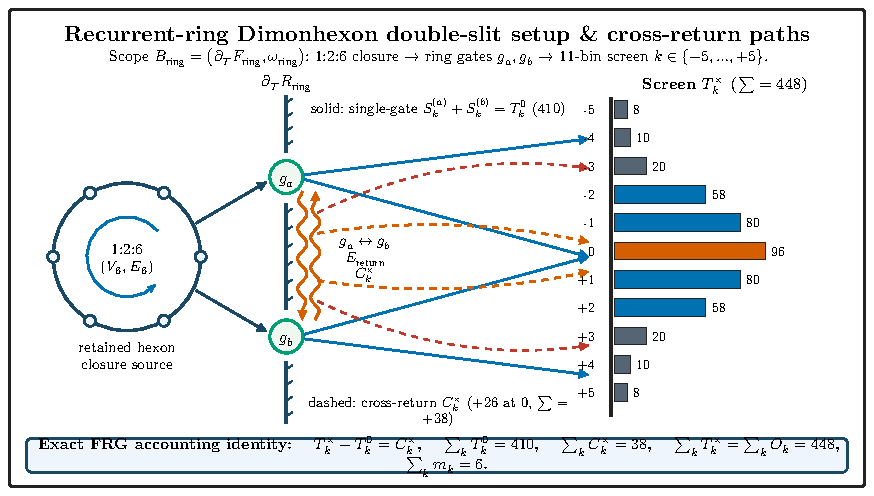
\includegraphics[width=0.92\linewidth,height=0.78\textheight,keepaspectratio]{figures/generated/double-slit-cross-return-setup.pdf}
\caption{Recurrent-ring double-slit cross-return setup. Two boundary gates produce independent one-gate contributions; the no-cross baseline is the sum of one-gate contributions, and the cross-return contribution produces the declared cross-return fixture.}
\label{fig:manual-recurrent-ring-double-slit}
\end{figure}

\paragraph{Derivation.}
The independent two-gate baseline is

\[
T^0_k=S^{(a)}_k+S^{(b)}_k.
\]

Summing coupled paths across the bound discrete-window cut dummy $t\in\omega$
(distinct from target bin $k\in K_{\mathrm{bin}}$) defines the cross-return term

\[
C^{\times}_k(B)=C_{ab,k}^{\times}(B)=\sum_{t\in\omega}\sum_{\gamma:g_a\leftrightarrow g_b\leadsto k}\kappa_k\SADARop_{B|t}(C_{\gamma}).
\]

Adding the baseline and cross-return yields the recurrent ring value

\[
T^{\times}_k=T^0_k+C^{\times}_k,
\]

and therefore the exact bin-level audit identity

\[
\boxed{T^{\times}_k-T^0_k=C^{\times}_k.}
\]

\subsubsection{Exact double-slit fixture}\label{manual:cross-return:exact-double-slit-fixture}

\paragraph{Specialization (\texttt{RC-030}).}
The released A$\Omega$-internal integer-bin fixture compares the recurrent ring value
$T_k^{\times}=T_k^0+C_k^{\times}$ against the declared comparator $O_k$ via the
exact signed residual $\Delta^{\mathbb{Z}}_k=T^{\times}_k-O_k$ and ternary tally
$\delta_{3,k}(T^{\times},O)=(s_k^{(3)},m_k)$.

\begin{table}[H]
\centering
\caption{Dimonhexon slit handoff: exact $\delta_3$ reclosure-bin fixture (\texttt{RC-030}).}
\label{tab:manual-dimonhexon-double-slit-fixture}
{\footnotesize
\begin{tabular}{rrrrrrrr}
\toprule
$k$ & $S_k$ & $T^0_k$ & $C^{\times}_k$ & $T^{\times}_k$ & $O_k$ & $\Delta^{\mathbb{Z}}_k$ & $\delta_{3,k}$ \\
\midrule
$-5$ & 4 & 8 & 0 & 8 & 8 & 0 & $(0,0)$ \\
$-4$ & 9 & 18 & -8 & 10 & 11 & -1 & $(-1,1)$ \\
$-3$ & 16 & 32 & -12 & 20 & 19 & 1 & $(+1,1)$ \\
$-2$ & 25 & 50 & 8 & 58 & 59 & -1 & $(-1,1)$ \\
$-1$ & 31 & 62 & 18 & 80 & 79 & 1 & $(+1,1)$ \\
$0$ & 35 & 70 & 26 & 96 & 95 & 1 & $(+1,1)$ \\
$1$ & 31 & 62 & 18 & 80 & 80 & 0 & $(0,0)$ \\
$2$ & 25 & 50 & 8 & 58 & 58 & 0 & $(0,0)$ \\
$3$ & 16 & 32 & -12 & 20 & 21 & -1 & $(-1,1)$ \\
$4$ & 9 & 18 & -8 & 10 & 10 & 0 & $(0,0)$ \\
$5$ & 4 & 8 & 0 & 8 & 8 & 0 & $(0,0)$ \\
\bottomrule
\end{tabular}
}
\end{table}

Here $C^{\times}_k=T^{\times}_k-T^0_k$. At the center bin ($k=0$),

\[
T^{\times}_0=96,\qquad O_0=95,\qquad\Delta^{\mathbb{Z}}_0=1,\qquad\delta_{3,0}=(+1,1),
\]

and across all eleven bins $k\in\{-5,\dots,+5\}$,

\[
\sum_kT_k^{\times}=448,\qquad\sum_kO_k=448,\qquad\sum_k\Delta^{\mathbb{Z}}_k=0,\qquad\sum_km_k=6.
\]

\begin{figure}[H]
\centering
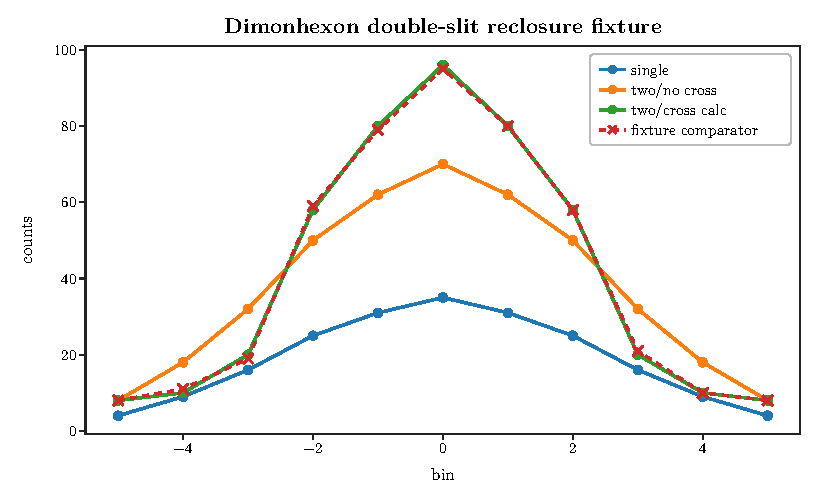
\includegraphics[width=0.92\linewidth,height=0.78\textheight,keepaspectratio]{figures/generated/double-slit-reclosure-fixture.pdf}
\caption{Dimonhexon double-slit reclosure fixture (\texttt{RC-030}). Cross-return changes the two-gate distribution; the exact internal comparison is recorded by $\delta_3$.}
\label{fig:manual-double-slit-reclosure-fixture}
\end{figure}

\begin{table}[H]
\centering
\caption{Recurrent-ring cross-return symbol table.}
\label{tab:manual-recurrent-ring-symbols}
{\footnotesize
\begin{tabular}{ll}
\toprule
Symbol & Meaning \\
\midrule
$S^{(a)}_k$ & one-gate contribution from $g_a$ into bin $k$ \\
$S^{(b)}_k$ & one-gate contribution from $g_b$ into bin $k$ \\
$T^0_k$ & independent gate-sum value \\
$C_{ab,k}^{\times}(B)$ & cross-return contribution from $g_a\leftrightarrow g_b$ into bin $k$ \\
$T^{\times}_k$ & recurrent ring value \\
$O_k$ & declared fixture comparator, if used \\
$\Delta_k^{\mathbb{Z}}$ & exact signed integer fixture residual \\
$\delta_{3,k}(T^{\times},O)$ & exact ternary signed residual tally \\
\bottomrule
\end{tabular}
}
\end{table}

\aodnoteblock{Status}{Released A$\leftrightarrow\Omega$-internal field-ring fixture verified in exact zero-float ternary arithmetic (\texttt{RC-030}).}

\paragraph{Engine path-pair generator and physical-law separation.}
Vector \texttt{RC-030} genuinely executes the finite $C_6$ ($(V_6,E_6)$) two-step
path-pair generator (\texttt{frg\_dimonhexon\_double\_slit\_ring}, tabulated in
\texttt{manual/data/boundary\_sadar/dimonhexon\_double\_slit\_ring\_paths.csv} and
verified by \texttt{python3 -B -m manual.engine --sector boundary\_sadar} and
\texttt{aod-core --verify-vectors --check-zero-float}) across symmetric gates
$g_a=-2,g_b=+2$ and bins $k\in\{-5,\dots,+5\}$ in exact
zero-float \texttt{TritWord}/\texttt{TritRatio} arithmetic: single-gate path pairs
burn contiguous optional dwell (\texttt{00} / $0_D$) under hexon aperture
saturation live via \texttt{TritWord.burn\_contiguous\_dwell} while preserving the
mandatory structural hinge (\texttt{11} / $0_H$), two-gate cross-return pairs
pack into 4-bit \texttt{ChiralPair4} registers, and exact summation reproduces
$\sum_kT^0_k=410$, $\sum_kC^{\times}_k=38$,
$\sum_kT^{\times}_k=448$ ($410+38=448$), $\sum_k\Delta^{\mathbb{Z}}_k=0$, and
$\sum_km_k=6$.

External physical detector and exposure probability laws remain strictly separated
from this internal path-pair generator. Signed internal contributions are not
physical probabilities: any downstream empirical comparison must declare separate
detector, loss/throughput, and exposure rules distinguishing expected counts,
unconditional detection including loss, and detected-bin conditional normalization
so normalization never erases throughput.

\aodprovenance{\mainsection{main:subsec:fractal-field-ring-gate};
\mainequation{main:eq:b-scoped-flux};
\mainequation{main:eq:frg-cross-return-contribution};
\secref{manual:cross-return:dimonhexon-slit}.}

\aodremark{The independent gate-sum value records independent reclosure; the recurrent ring value records redistributed returned-current coupling.}

\subsection{Short-window fixture scope}\label{manual:short-window:scope}

\aodnoteblock{Scope}{This section is A$\Omega$-internal. It tests short-window $\rho^D$-clipping, pending overhang, closure residual, and sheddic path status without external comparison.}

\paragraph{Setup.}
Declare the short-window fixture scope

\[
\mathbf{a}_{\mathrm{sw}}\vdash(F_{\mathrm{sw}},R_{\mathrm{sw}},\partial R_{\mathrm{sw}},\omega_{\mathrm{sw}}),\qquad B_{\mathrm{sw}}=(\partial F_{\mathrm{sw}},\omega_{\mathrm{sw}}).
\]

\paragraph{Duration-domain declaration.}
These reductions declare $R^{\mathrm{asym}}=\mathrm{id}$ and the additive
native count realization, so $\rho^D=RD$ in this specialization. The window is a
count in that same domain, giving scalar participation
$\rho^D_{\omega}=\min(\rho^D,|\omega|)$; neither structural support
$RD$ nor the coupled $\mathrm{RCD}$ object is clipped. The baseline Dimonon
support used below is

\[
\Pi(1:2)=2^1+2=4,\qquad H_{\mu}=1,\qquad\rho^D_{1:2}=RD^{(1)}(1:2)=2\cdot4+1=9,
\]

while record length $L_M$ remains distinct from path-derived scalar $\rho^D$.

\begin{figure}[H]
\centering
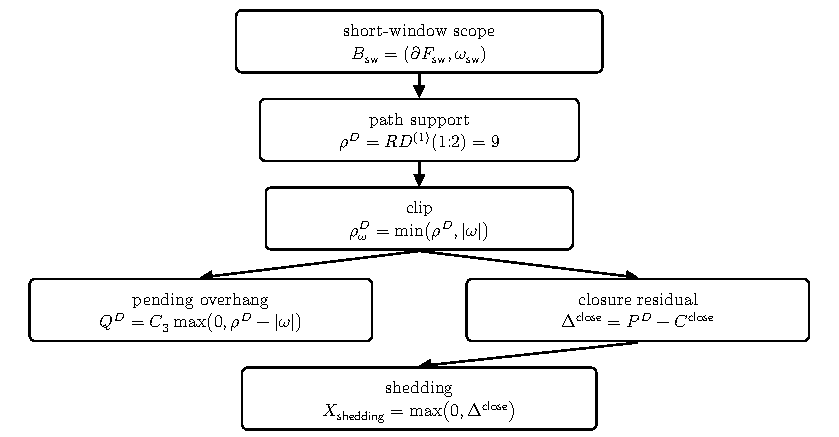
\includegraphics[width=\linewidth]{figures/generated/short-window-setup.pdf}
\caption{Short-window RCD fixture flow. The path-derived $\rho^D$ is clipped by the declared window to produce $\rho^D_{\omega}$, while pending overhang $Q^D$ and closure residual $\Delta^{\mathrm{close}}$ are kept separate from shedding excess.}
\label{fig:manual-short-window-setup}
\end{figure}

\subsection{Shared fixture equations}\label{manual:short-window:equations}

\paragraph{Derivation.}
For a candidate record $M$ in declared scope $B$, evaluate the five exact integer
quantities:

\[
\rho^D_{\omega}(M;B)=\min(\rho^D(M;B),|\omega|),
\]

\[
Q^D(M;B)=C_3\max(0,\rho^D(M;B)-|\omega|),
\]

\[
P^D(M;B)=C_3\rho^D_{\omega}(M;B),
\]

\[
\Delta^{\mathrm{close}}(M;B)=P^D(M;B)-C^{\mathrm{close}}(M;B),
\]

\[
X_{\mathrm{shedding}}(M;B)=\max(0,\Delta^{\mathrm{close}}(M;B)).
\]

\aodnoteblock{Remark}{$\Delta^{\mathrm{close}}$ records signed closure residual, whereas $X_{\mathrm{shedding}}$ records nonnegative surplus only. Negative closure residuals remain deficits or open checks, never sheddic surplus.}

\subsection{Closure-dependent and surplus fixtures}\label{manual:short-window:fixture-table}

Keeping $\Delta^{\mathrm{close}}$ and $X_{\mathrm{shedding}}$ distinct prevents
closure-deficit records from being misread as sheddic surplus.

\begin{table}[H]
\centering
\caption{Short-window RCD and shedding fixtures. All records use $C_3=3$ and $\rho^D=RD^{(1)}(1:2)=9$.}
\label{tab:manual-short-window-fixtures}
{\footnotesize
\begin{tabular}{cccccccccc}
\toprule
Row & $C_3$ & $\rho^D$ & $L_M$ & $|\omega|$ & $\rho^D_{\omega}$ & $Q^D$ & $P^D$ & $C^{\mathrm{close}}$ & $\Delta^{\mathrm{close}},X_{\mathrm{shedding}}$ \\
\midrule
$1:2:7\to C_6$ & 3 & 9 & 7 & 7 & 7 & 6 & 21 & 18 & $3,3$ \\
$1:2:7\to C_8$ & 3 & 9 & 7 & 7 & 7 & 6 & 21 & 24 & $-3,0$ \\
$1:2:9\to C_8$ & 3 & 9 & 9 & 9 & 9 & 0 & 27 & 24 & $3,3$ \\
$1:2:10\to C_{10}$ & 3 & 9 & 10 & 10 & 9 & 0 & 27 & 27 & $0,0$ \\
\bottomrule
\end{tabular}
}
\end{table}

\subsection{The \texorpdfstring{$1:2:7$}{1:2:7} closure-dependent fixture}\label{manual:short-window:127}

For $1:2:7$, the window is shorter than path-derived support:

\[
\rho^D_{\omega}=\min(9,7)=7,\qquad Q^D=3(9-7)=6,\qquad P^D=3\cdot7=21.
\]

Against lower closure $C_6=18$, the fixture carries surplus ($\Delta^{\mathrm{close}}=3$, $X_{\mathrm{shedding}}=3$):

\[
\Delta^{\mathrm{close}}=21-18=3,\qquad X_{\mathrm{shedding}}=3,
\]

whereas against upper closure $C_8=24$, it is closure-deficient:

\[
\Delta^{\mathrm{close}}=21-24=-3,\qquad X_{\mathrm{shedding}}=0.
\]

Hence $1:2:7$ is closure-dependent.

\subsection{The \texorpdfstring{$1:2:9$}{1:2:9} surplus fixture}\label{manual:short-window:129}

For $1:2:9$, the window matches full path-derived support:

\[
\rho^D_{\omega}=\min(9,9)=9,\qquad Q^D=0,\qquad P^D=3\cdot9=27.
\]

Against $C_8=24$,

\[
\Delta^{\mathrm{close}}=27-24=3,\qquad X_{\mathrm{shedding}}=3,
\]

producing the nine-window surplus fixture.

\subsection{The \texorpdfstring{$1:2:10$}{1:2:10} clipped retained fixture}\label{manual:short-window:1210}

For $1:2:10$, candidate record length exceeds path-derived support, so clipping
caps participation at $9$:

\[
\rho^D_{\omega}=\min(9,10)=9,\qquad Q^D=0,\qquad P^D=27.
\]

Against $C_{10}=27$,

\[
\Delta^{\mathrm{close}}=0,\qquad X_{\mathrm{shedding}}=0,
\]

yielding a clipped retained check.

\subsection{Sheddic path audit}\label{manual:short-window:shedpath-audit}

\paragraph{Falsification and witness ordering.}
The sheddic path audit requires an explicit target channel from

\[
\mathrm{SheddicPath}(X_{\mathrm{shedding}})\in\{E_2,\mathsf{C}_6,\mathsf{C}_8,\mathsf{C}_{10},\dots,\mathsf{C}_{2n}\}.
\]

The four pressure tuples above supply amounts only. Complete routing must separately
bind route identity, allocated amount, conservation, and---whenever retention is
claimed---a retained-form and lifetime/window witness; positive surplus alone supplies
none of those certificates. When a routed surplus emits a shed continuation
(\mainequation{main:eq:shed-continuation-witness}), downstream delivery, acceptance,
seating, initial recipient origin closure, and later compatible reclosure remain
separate witness-ordered stages (\mainequation{main:eq:recipient-event-lattice});
routed surplus alone proves no recipient reclosure. A missing route leaves that stage
incomplete, and a deficit remains an open check unless a declared closure completion
is supplied.

\subsection{Audit hooks}\label{manual:short-window:audit-hooks}

\aodnoteblock{Audit}{Every short-window fixture records $\rho^D_{\omega}$, $Q^D$, $\Delta^{\mathrm{close}}$, and $X_{\mathrm{shedding}}$ separately. Sheddic surplus is nonnegative only; completed routing additionally requires a declared sheddic path and its conservation witness.}

\aodprovenance{\mainequation{main:eq:window-clipped-rho};
\mainequation{main:eq:burden-overhang};
\mainequation{main:eq:sheddic-path};
\mainequation{main:eq:shed-continuation-witness};
\mainequation{main:eq:recipient-event-lattice};
\secref{manual:short-window:scope}.}

\aodremark{This section is A$\Omega$-internal: it prepares the exact clipping and conservation mechanics reused by rest-energy and boundary-current records without introducing an external comparison target.}

\subsection{Five-boundary short-window clipping and shedding D.E.C. ledger}\label{manual:short-window:dec-clipping-ledger}

\paragraph{Setup and engine verification (\texttt{RC-038}).}
Declare the short-window clipping and enclosure boundary stack

\[
B_{\mathrm{core}}\to B_{\omega}\to B_{\mathrm{close}}\to B_{\mathrm{shed}}\to B_{\mathrm{ext}}.
\]

Vector \texttt{RC-038} (\texttt{dec\_short\_window\_rcd\_clipping}), verified alongside
\texttt{RC-030} by \texttt{python3 -B -m manual.engine --sector boundary\_sadar} and
\texttt{aod-core --verify-vectors --check-zero-float} in
\texttt{manual/data/boundary\_sadar/short\_window\_rcd\_dec\_ledger.csv}, evaluates exact
single-channel window clipping $\rho^D_{\omega}=\min(RD,|\omega|)$,
active pressure $p^D=3\rho^D_{\omega}$, pending overhang
$Q^D=3\max(0,RD-|\omega|)$, and odd-window shedding
$X_{\mathrm{shedding}}=\max(0,p^D-C_{\mathrm{close}})$ across $1:2$
($RD=9$), $3:3$ ($RD=61$), and $3:4$ ($RD=137$). Every row satisfies
exact integer conservation $p^D+Q^D=3RD$ ($27$, $183$, and $411$), while
positive shedding $X_{\mathrm{shedding}}=3$ activates uniquely on the full odd
Dimonon window $(1:2,|\omega|=9)$ exceeding $\mathsf{C}_8=24$.

\begin{figure}[H]
\centering
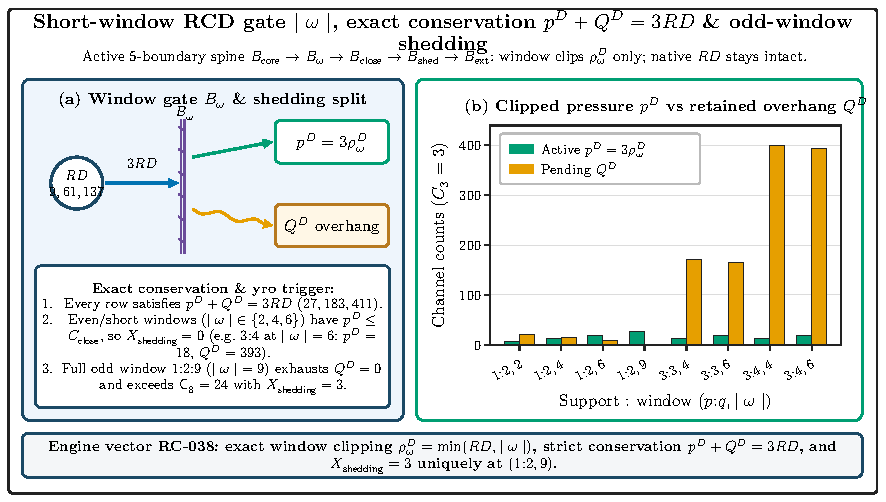
\includegraphics[width=0.92\linewidth,height=0.78\textheight,keepaspectratio]{figures/generated/short-window-boundary-feynman.pdf}
\caption{Short-window boundary gate $B_{\omega}$ clipping $3RD$ into active pressure $p^D=3\rho^D_{\omega}$ and retained overhang $Q^D$ with exact conservation $p^D+Q^D=3RD$ (\texttt{RC-038}, \texttt{short\_window\_rcd\_dec\_ledger.csv}).}
\label{fig:manual-short-window-boundary-feynman}
\end{figure}

\begin{table}[H]
\centering
\caption{Engine-bound short-window RCD clipping, overhang conservation, and odd-window shedding D.E.C. ledger (\texttt{RC-038}, live from \texttt{short\_window\_rcd\_dec\_ledger.csv}).}
\label{tab:manual-short-window-dec-ledger}
{\footnotesize
\begin{tabular}{>{\raggedright\arraybackslash}p{0.088\linewidth}>{\raggedleft\arraybackslash}p{0.072\linewidth}>{\raggedleft\arraybackslash}p{0.076\linewidth}>{\raggedleft\arraybackslash}p{0.076\linewidth}>{\raggedleft\arraybackslash}p{0.072\linewidth}>{\raggedleft\arraybackslash}p{0.080\linewidth}>{\raggedleft\arraybackslash}p{0.092\linewidth}>{\raggedleft\arraybackslash}p{0.124\linewidth}>{\raggedleft\arraybackslash}p{0.120\linewidth}}
\toprule
Support & $RD$ & $|\omega|$ & $\rho^D_{\omega}$ & $p^D$ & $Q^D$ & $C_{\mathrm{close}}$ & $X_{\mathrm{shedding}}$ & $p^D+Q^D$ \\
\midrule
1:2 & 9 & 2 & 2 & 6 & 21 & 18 & 0 & 27 \\
1:2 & 9 & 4 & 4 & 12 & 15 & 18 & 0 & 27 \\
1:2 & 9 & 6 & 6 & 18 & 9 & 18 & 0 & 27 \\
1:2 & 9 & 9 & 9 & 27 & 0 & 24 & 3 & 27 \\
3:3 & 61 & 4 & 4 & 12 & 171 & 18 & 0 & 183 \\
3:3 & 61 & 6 & 6 & 18 & 165 & 18 & 0 & 183 \\
3:4 & 137 & 4 & 4 & 12 & 399 & 18 & 0 & 411 \\
3:4 & 137 & 6 & 6 & 18 & 393 & 18 & 0 & 411 \\
\bottomrule
\end{tabular}
}
\end{table}
